\documentclass[12pt]{article}
% Formatting
\usepackage[letterpaper,margin=1.0in, footskip=30pt]{geometry}
\renewcommand{\baselinestretch}{1.0}
% Symbols
\usepackage[T1]{fontenc} % For accidents characters
% Mathematics 
\usepackage{amsmath} 
% Theorems
\usepackage{amsthm}
\newtheorem{theorem}{Theorem}
% Figures
\usepackage{graphicx} % For images
\graphicspath{{figs}} % So that images can be stored in the directory `figs`
\usepackage{float} % For positioning figures
\usepackage{tikz} % For shapes
\usepackage{tikz-cd} % For commutative diagrams
% Bibliography
\usepackage[backend=biber]{biblatex}
\addbibresource{refs.bib}
% 
\title{Latex Template}
\author{Dustin Enyeart}
\date{17 October 2024}
% 
\begin{document}


\maketitle % Add title, author and date

\section{Example Section}

\subsection{Example Subsection}

This $2+2$ is some in-line mathematics. 
This 
\[
    \sum_{i=1}^n \frac{1}{i^2} = \frac{\pi^2}{6}
\]
is some out-of-line mathematics.
This
\[
    \begin{pmatrix}
    1 & 2 \\
    3 & 4 \\
    \end{pmatrix}
\]
is a matrix. 


\begin{theorem}
This is a theorem.
\end{theorem}
\label{thm:example}

\begin{proof}
This is a proof. 
\end{proof}

Theorem \ref{thm:example} is an example of an internal reference.
And, external references can be use with bibtex \cite{feynman2014qed, vaswani2017attention, enyeart2024latex}. 

\begin{figure}[H]
    \centering
    \includegraphics[width=0.5\textwidth]{fig1.png}
    \caption{Example Image}
\end{figure}


\begin{table}
    \centering
    \caption{Example Table}
    \begin{tabular}{c|c|c}
        Column 1 & Column 2 & Column 3 \\ \hline
        A & B & C \\ \hline
        D & E & F \\ \hline
        G & H & I \\ 
    \end{tabular}
    \label{tab:example}
\end{table}


Here is a shape. 


\begin{center}
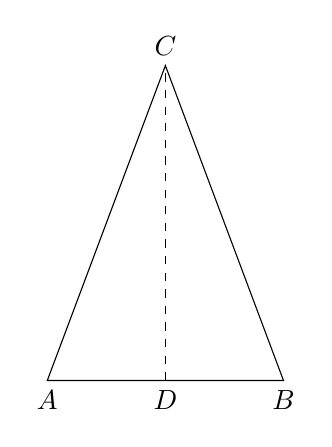
\begin{tikzpicture}
    \draw (0,0) node[below]{$A$}
    -- (3,0) node[below]{$B$}
    -- (1.5,4) node[above]{$C$}
    -- cycle;
    \draw[dashed] (1.5,0) node[below]{$D$} -- (1.5, 4);
\end{tikzpicture}
\end{center}


Here is a commutative diagram. 

\[
\begin{tikzcd}
    G \arrow{dr} \arrow{rr}{f} & & G' \\
    & G/H \arrow{ur} & \\
\end{tikzcd}
\]


\printbibliography % Add bibliography


\end{document}